% %% %%%%%%%%%%%%%%%%%%%%%%%%%%%%%%%%%%%%%%%%%%%%%%%%%%%%%%%%%%
% intro-zerox.tex
%
% Author:  Mauricio Matamoros
% License: MIT
%
% %% %%%%%%%%%%%%%%%%%%%%%%%%%%%%%%%%%%%%%%%%%%%%%%%%%%%%%%%%%%
%!TEX root = ../practica.tex
%!TEX root = ../references.bib

% CHKTEX-FILE 1
% CHKTEX-FILE 13
% CHKTEX-FILE 46

\subsection{Detector de cruce por cero}%
\label{seq:intro-zeroX}
Un circuito detector de cruce por cero es un circuito electrónico diseñado para detectar cuando una señal senoidal pasa por cero.
Estos circuitos se usan comunmente en electrónica de potencia tanto para detectar la frecuencia de la línea y hacer cálculo de fases.
Además, al reducirse la diferencia de potencial a cero entre la fase y el neutro, la corriente instantánea también es cero, haciendo de éste el momento ideal para cortar la alimentación sin dañar las cargas.

\begin{figure}[H]
	\centering
	\begin{subfigure}[b]{0.5\columnwidth}
		\centering
		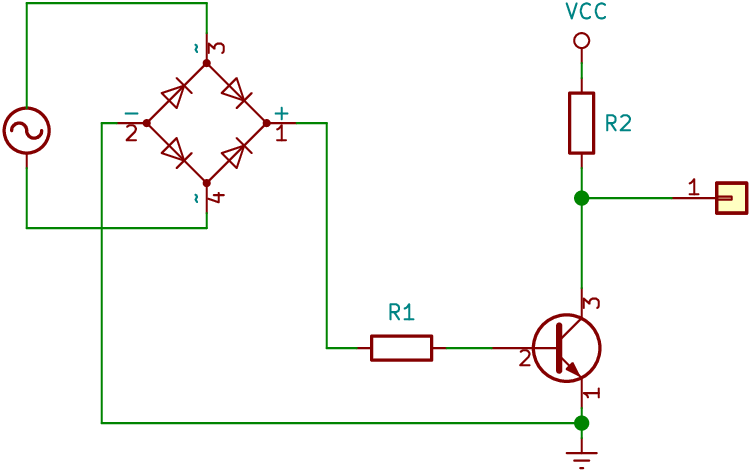
\includegraphics[width=\textwidth,height=5cm,keepaspectratio]{img/zcross-1.png}
		\caption{Detector de cruce por cero simple}
		\label{fig:zx1} %chktex 24
	\end{subfigure}%
	\begin{subfigure}[b]{0.5\columnwidth}
		\centering
		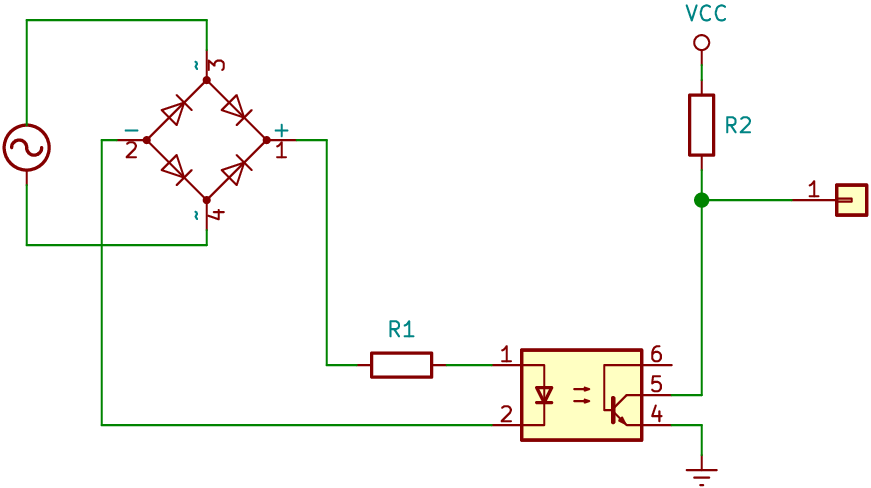
\includegraphics[width=\textwidth,height=5cm,keepaspectratio]{img/zcross-2.png}
		\caption{Detector de cruce por cero optoacoplado}
		\label{fig:zx2} %chktex 24
	\end{subfigure}
	\caption{Detectores de cruce por cero}
	\label{fig:zx} % chktex 24
\end{figure}

La forma más sencilla de alambrar un circuito detector de cruce por cero es mediante un puente rectificador, dos resistencias y un transistor tipo NPN en modo interruptor (véase~\Cref{fig:zx1}).
El puente rectificador se encarga de invertir la parte negativa de la señal de AC, evitando así corrientes inversas que el transistor es incapaz de manejar.
Cuando hay voltaje en la línea, éste habilita la base cerrando el circuito del transistor y conectando el pin de sensado a tierra (la resistencia de base evita el corto circuito y ajusta el umbral de sensibilidad).
Tan pronto como la diferencia de potencial entre la línea y el neutro cae a cero (o suficientemente bajo como la resistencia de base permita) el circuito se abre y en el pin de sensado se registra \textsc{Vcc}.

Para calcular $R_1$ es necesario tomar en cuenta las características eléctricas del transistor y los voltajes de pico de la línea.
Se sabe que $V_\text{pico}=V_\text{RMS}\sqrt{2}$, por lo que usando la ley de ohm se tiene:
\begin{equation}
	R_1 = \frac{V_\text{RMS}\sqrt{2}}{i_\text{transistor}} \approx
	\frac{1.4142V_\text{RMS}}{i_\text{transistor}}
\end{equation}

Sin embargo, el voltaje de la línea rara vez viene rectificado y un transitorio de corriente derivado de una descarga inductiva (arranque de refrigerador o microondas) puede incluso duplicar el voltaje de la línea, quemando no sólo el transistor sino el microprocesador.
Es por esto que es muy aconsejable utilizar un optoacoplador en lugar de un simple transistor, tal como muestra la figura \Cref{fig:zx2}.
Los principios de operación son los mismos.
